\RequirePackage{xcolor}
\documentclass{ieeeaccess}
\usepackage{cite}
\usepackage{amsmath,amssymb,amsfonts}
\usepackage{algorithmic}
\usepackage{graphicx}
\usepackage{textcomp}
\usepackage{booktabs}
\usepackage{multirow}
\usepackage{hyperref}
\usepackage{svg}

% Redefinição de cores obrigatória para evitar o erro "undefined access blue" na classe ieeeaccess
\definecolor{accessblue}{cmyk}{1,0.49,0,0}
\definecolor{greycolor}{cmyk}{0,0,0,0.8}

\usepackage{bm}
\makeatletter
\AtBeginDocument{\DeclareMathVersion{bold}
\SetSymbolFont{operators}{bold}{T1}{times}{b}{n}
\SetSymbolFont{NewLetters}{bold}{T1}{times}{b}{it}
\SetMathAlphabet{\mathrm}{bold}{T1}{times}{b}{n}
\SetMathAlphabet{\mathit}{bold}{T1}{times}{b}{it}
\SetMathAlphabet{\mathbf}{bold}{T1}{times}{b}{n}
\SetMathAlphabet{\mathtt}{bold}{OT1}{pcr}{b}{n}
\SetSymbolFont{symbols}{bold}{OMS}{cmsy}{b}{n}
\renewcommand\boldmath{\@nomath\boldmath\mathversion{bold}}}
\makeatother

\def\BibTeX{{\rm B\kern-.05em{\sc i\kern-.025em b}\kern-.08em
    T\kern-.1667em\lower.7ex\hbox{E}\kern-.125emX}}

% \usepackage{orcidlink}
% \PassOptionsToPackage{bookmarks=false}{hyperref} %Used so orcidlink does not lead to bookmark creation
% \hypersetup{hidelinks} %Used so no box around orcidlinks


%Your document starts from here ___________________________________________________
\begin{document}
\history{Date of publication xxxx 00, 0000, date of current version xxxx 00, 0000.}
\doi{10.1109/ACCESS.2026.0429000}

\title{Evaluation of Indices for Monitoring the Voltage Stability Margin of Power Systems}

\author{\uppercase{Gonçalo Fontenele}\authorrefmark{1}, \uppercase{Leonardo Rafael Bergonci Campos}\authorrefmark{1}, and
	\uppercase{Murilo E. C. Bento}\authorrefmark{1}, \IEEEmembership{Member, IEEE}}

\address[1]{Department of Electrical Engineering, Federal University of Rio de Janeiro, Rio de Janeiro, RJ 21941-909, Brazil (e-mails: goncalogfb@poli.ufrj.br, bergoncileo@gmail.com, murilobento@poli.ufrj.br)}
\tfootnote{This work was supported in part by the Coordination for the Improvement of Higher Education Personnel—CAPES under Grant 00x0ma614 and Grant 001, in part by the Conselho Nacional de Desenvolvimento Científico e Tecnológico (CNPq).}

\markboth
{Fontenele, G. \headeretal: Evaluation of Indices for Monitoring the Voltage Stability Margin}
{Fontenele, G. \headeretal: Evaluation of Indices for Monitoring the Voltage Stability Margin}

\corresp{Corresponding author: Murilo E. C. Bento (e-mail: murilobento@poli.ufrj.br).}

\begin{abstract}
Voltage stability is a fundamental requirement for the secure operation of power systems, especially in operational scenarios close to transmission limits. This paper presents the development of a Python-based computational tool utilizing the Pandapower library for static voltage stability margin analysis. A Continuation Power Flow (CPF) algorithm featuring an adaptive step size strategy and distributed slack generation dispatch was implemented, designed to accurately replicate the solution methodology of the ANAREDE commercial software. The study validates the tool through a rigorous cross-comparison with ANAREDE using the IEEE 30-bus system, demonstrating negligible deviations. Furthermore, the tool's flexibility and adaptability are demonstrated on the IEEE 39-bus New England system. Additionally, a detailed comparative analysis of multiple Voltage Stability Indices (VSIs), such as FVSI, $L_{mn}$, NLSI, NVSI, and the L-index, is performed, showcasing the correlation between these indicators and the imminence of voltage collapse.
\end{abstract}

\begin{keywords}
Power Systems, Power System Stability, Voltage Stability, Continuation Power Flow, Stability Indices, Pandapower, ANAREDE.
\end{keywords}

\titlepgskip=-21pt

\maketitle

\section{Introduction}
\label{sec:introduction}

\PARstart{T}{he} evolution of power systems has increasingly posed significant challenges to operation centers worldwide \cite{Bhusal2020}. Growing uncertainty in hourly demand, the large-scale integration of intermittent renewable energy sources such as wind and photovoltaic generation, the increasing occurrence of equipment failures and extreme weather conditions, including temporary and permanent short circuits, and the vulnerability of communication infrastructures to cyberattacks all add substantial complexity to the continuous and secure operation of modern power systems \cite{Pastrana2025,Rifat2025,AlRousan2025,Manias2024,Ali2024,Hashemi2025}. These emerging challenges underscore the need for new and effective tools to support operation centers in maintaining system reliability, resilience, and operational security.

Power system stability studies have become an essential task to ensure the safe and proper functioning of modern power systems \cite{Hatziargyriou2021}. Voltage stability assessment has gained prominence due to the increasingly stressed operation of power systems, driven by rising demand and the integration of renewable energy sources far from load centers \cite{Sun2019}. Voltage collapse, characterized by a progressive and uncontrollable drop in voltage levels across a significant portion of the system, is frequently associated with the inability of the transmission network and generators to meet the reactive power requirements of the load \cite{kundur1994power,cutsem2007voltage}.

To determine the security margin up to the point of collapse (known as the ``nose'' of the PV curve), the industry widely employs the Continuation Power Flow (CPF) \cite{Ajjarapu1992}. Determining the point of maximum power transfer allows us to formulate the Voltage Stability Margin (VSM), which is the difference between the power levels in the nominal case and the case of maximum power transfer. Commercial software, such as ANAREDE (developed by CEPEL) in Brazil \cite{cepel2009anarede}, uses robust methods to bypass the singularity of the Jacobian matrix at the maximum transfer point. Reproducing these methods in an open academic environment is essential for developing new analytical metrics and control algorithms. The literature shows that determining the security margin in voltage stability studies remains a challenging task, which has motivated the continuous development of new methodologies aimed at overcoming existing limitations. In addition to the Continuation Power Flow method \cite{Ajjarapu1992}, the scientific community has proposed approaches based on Thévenin theory \cite{Corsi2008}, eigenvalue analysis \cite{Bento2018}, and, more recently, machine learning techniques such as Artificial Neural Networks \cite{Zhou2010}, Graph Neural Networks \cite{Guddanti2023}, and Decision Trees \cite{Meng2020}.

The growth and evolution of information technologies, sensors, and communication, along with their integration into power systems, have led to the development of smart grids \cite{Li2010}. Phasor Measurement Units (PMUs) are smart grid devices capable of measuring voltage and current at their installation locations with good sampling rates \cite{Li2010}. Thus, a large number of well-located PMUs ensures greater real-time observability of power systems. The scientific community has evaluated the potential of PMU data in monitoring, control, and protection applications for power systems, and the proposals have shown significant improvements in system operation \cite{Ippolito2024,Bento2024,Shazdeh2023,Wang2024}.

PMU data have shown promise in various voltage stability analysis and control applications. Secondary voltage control using PMU data improves system regulation and ensures good dynamic system performance values \cite{Pierrou2024,Su2018,Chiodo2024}. A relevant set of voltage stability indices have been developed to assess the proximity of the operating point of an instability mechanism such as voltage collapse \cite{modarresi2016comprehensive}. These indices can use only PMU measurements or formulate Thevenin equivalents of the system at points of interest \cite{Pourbagher2022,Lee2019}.

There are requirements that must be established beforehand to determine the maximum power transfer and thus the Voltage Stability Margin. These requirements include (i) the nominal operating point of the system, (ii) the direction of load growth, (iii) the generation redispatch model and (iv) the topology of the electrical grid. However, in the real-time operation of power systems, all four of these requirements may differ from the previously established values, and thus the calculated VSM may be inadequate for the actual power system. In \cite{Bento2018b}, the authors showed that VSM values can be substantially reduced with variations in the direction of load growth and this index needs to be recalculated. There is a need for an approach to monitoring and evaluating the VSM considering both predicted and real-time scenarios. Most voltage stability indices were formulated to determine the maximum load level for one bus at a time in the system. However, the system load can increase collectively and not solely at one bus at a time. A preliminary analysis in \cite{madureira2023avaliacao} showed in a small-scale system that some voltage stability indices can indicate voltage instability problems for varying load levels and not only for the maximum load level of a given bus in the system. Thus, voltage stability indices and VSM have weaknesses that could be remedied with a combined approach. Voltage stability indices could be applied to monitor VSM and assess its suitability for real-world system scenarios.

This work proposes the development of a CPF simulator in Python \cite{thurner2018pandapower}, implementing step-size refinement and distributed generation dispatch techniques. The tool is rigorously validated by reproducing the reference results from \cite{madureira2023avaliacao} on the IEEE 30-bus system. Building upon this baseline, a comparative study is introduced using the larger, heavily meshed IEEE 39-bus New England system. This dual-system approach enables a critical comparative analysis of several Voltage Stability Indices (VSIs) reviewed by \cite{modarresi2016comprehensive}, illustrating how network topology affects the predictive capability of these metrics.

This article presents the following structure. Section \ref{sec:background} presents the theoretical foundation of voltage stability, voltage stability margin through the PV curve, and voltage stability indices. Section \ref{sec:tool} describes the Python computational tool used in this research. Section \ref{sec:method} presents the proposed methodology, highlighting the implementation resources. Section \ref{sec:results} presents the case studies and discussions carried out by applying the proposed method to IEEE test systems. Section \ref{sec:conclusions} concludes the article with the main analyses. Section \ref{sec:future} discusses future research directions.

\section{Theoretical Background}
\label{sec:background}

\subsection{Voltage Stability}
Voltage stability is the ability of a power system to maintain steady voltages at all buses after being subjected to a disturbance \cite{kundur1994power}. It is classified into:
\begin{itemize}
    \item \textbf{Large Disturbances:} The ability to maintain voltage after severe contingencies, such as the loss of generation or transmission circuits.
    \item \textbf{Small Disturbances:} The ability to control voltage in the face of slow load variations, which is the focus of this static study.
\end{itemize}

Collapse occurs when the system operates beyond the Maximum Power Transfer point, where the load impedance ($Z_{load}$) equals the Thevenin equivalent impedance of the network ($Z_{th}$). Mathematically, this point corresponds to a saddle-node bifurcation (SNB), where the Jacobian matrix of the power flow becomes singular, preventing the convergence of conventional methods (Newton-Raphson) \cite{cutsem2007voltage}.

\subsection{PV Curve}
A classic approach to visualizing the voltage collapse phenomenon is through the PV curve, which relates the active power demanded at a load bus (horizontal axis) to the corresponding voltage level (vertical axis). As the loading increases, the voltage tends to decrease gradually until it reaches a critical point where small additional load variations produce abrupt changes in voltage. This point, known as the Maximum Loading Point (MLP), represents the static limit of the system and coincides with the saddle-node bifurcation where the Jacobian matrix becomes singular.

The region preceding the MLP is characterized by stable operation, where for each power increment, a unique and physically consistent solution to the power flow exists. Past the MLP, no viable solution exists, implying that the system lacks the capacity to meet the imposed demand, leading to voltage collapse. The typical shape of the curve, often described as an inverted parabola, as shown in \autoref{fig:curva_pv}, evidences that the stability margin strongly depends on reactive power availability, network electrical characteristics, and the geographical location of the load.

The analysis of the PV curve is, therefore, fundamental for understanding voltage stability, as it allows for the direct identification of the point where the system ceases to operate safely. This graphical representation also serves as a reference for evaluating stability indices, which aim to approximately quantify the system's distance to this critical point.

\begin{figure}[htbp]
    \centering
    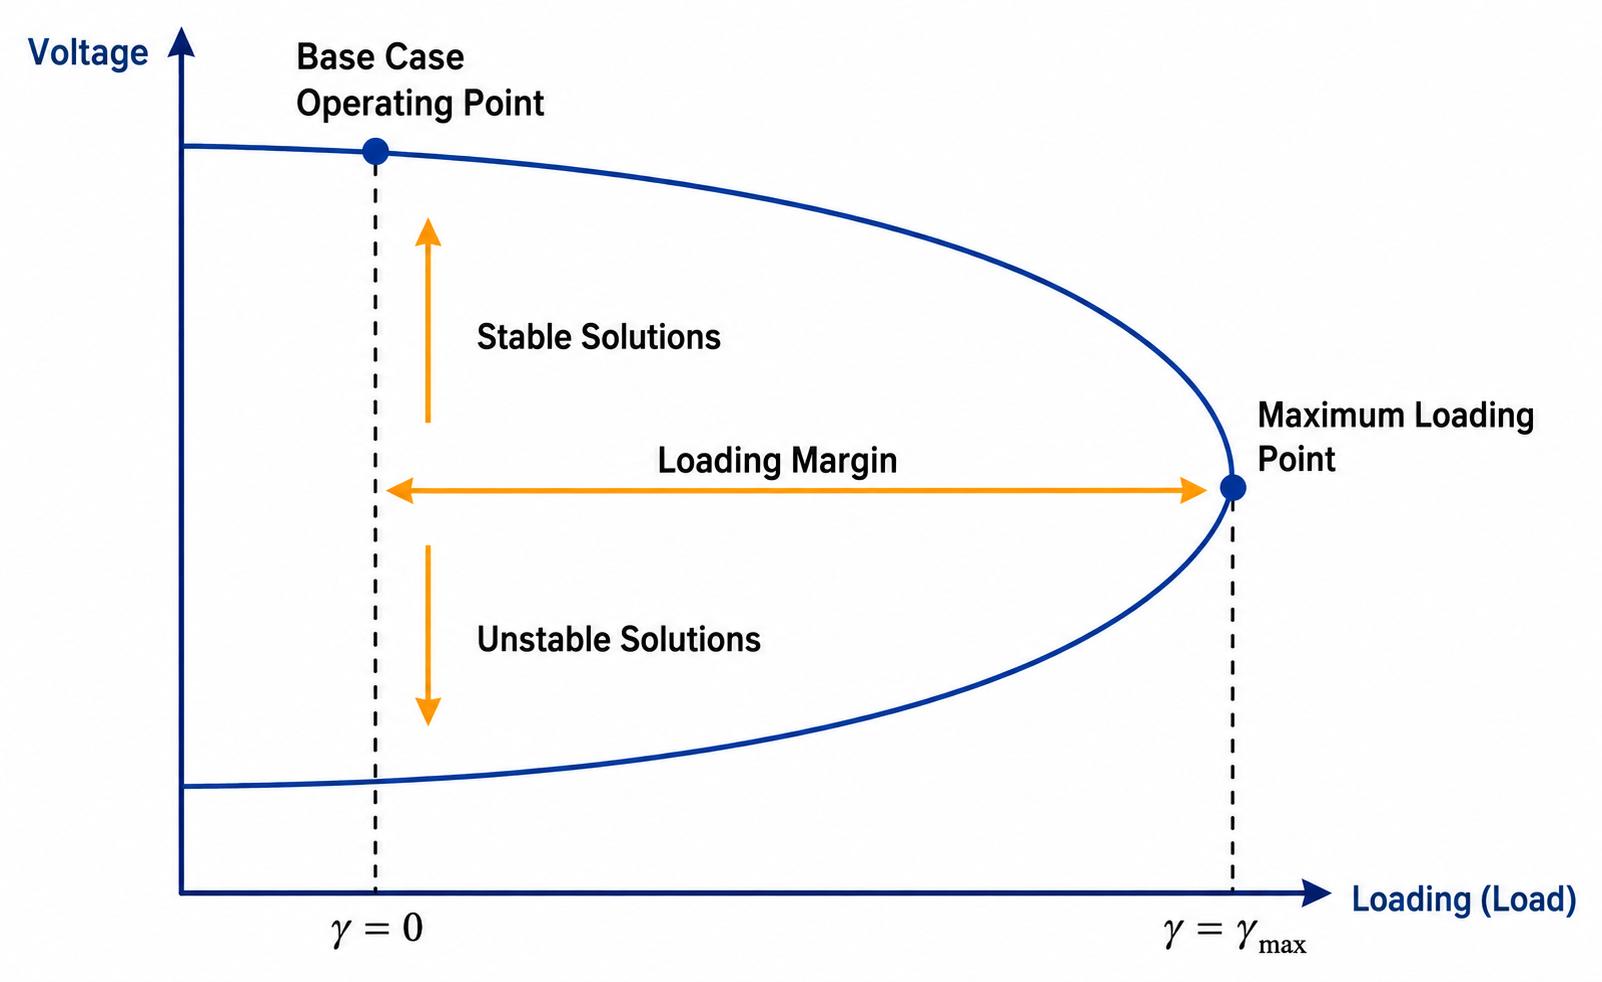
\includegraphics[width=\linewidth]{figures/curva_pv.png}
    \caption{Typical configuration of a PV curve, illustrating the voltage collapse phenomenon at the Maximum Loading Point (nose point) \cite{jaquelineresende2007}.}
    \label{fig:curva_pv}
\end{figure}

\subsection{Review of Voltage Stability Indices (VSIs)}
Voltage Stability Indices (VSIs) are scalar metrics used to quantify the degree of proximity of an electrical system to voltage collapse, reflecting the network's capacity to sustain adequate voltage levels under different loading conditions. Although each index adopts its own formulation and criteria, the general interpretation places them on a scale where values close to zero indicate safe operation and values close to one signal impending collapse. In this work, based on the comprehensive review presented by Modarresi et al.~\cite{modarresi2016comprehensive}, six indicators used in the literature are analyzed: the line indices FVSI, $L_{mn}$, NLSI, NVSI, and the nodal L-index.

\subsubsection{FVSI (Fast Voltage Stability Index)}
The FVSI is derived from the quadratic form of the power flow equations for a radial line, evaluating the proximity to the point where the equation ceases to have a real solution. Thus, the index expresses how close the system is to violating the discriminant condition $\geq 0$. Values close to 1 indicate that the reactive component of the load at the receiving bus is imposing significant stress on the line. Values greater than 1 indicate that one of the buses connected to the line may face a significant voltage drop, which could lead to a system collapse \cite{musirin2002}. 

For a line connecting bus $i$ (sending) to bus $j$ (receiving), it can be written as:
\begin{equation}
FVSI_{ij} = \frac{4 Z_{ij}^2 Q_j}{V_i^2 X_{ij}} \le 1.0
\end{equation}

\subsubsection{$L_{mn}$ (Line Stability Index)}
The $L_{mn}$ index utilizes the same concept as the FVSI regarding the requirement that the discriminant must be greater than or equal to zero to ensure stability, but it explicitly incorporates the angular dependence between the terminal voltages of the line. It evaluates the role of phase angle displacement and series impedance on stability. Lines with large power flows or heavily loaded lines tend to display small sine values in the denominator, amplifying the index.

Considering the line impedance angle $\theta$ and the angular displacement $\delta = \theta_i - \theta_j$ \cite{moghavvemi98}:
\begin{equation}
L_{mn} = \frac{4 X_{ij} Q_j}{(V_i \sin(\theta - \delta))^2} \le 1.0
\end{equation}

\subsubsection{NLSI (Novel Line Stability Index)}
Proposed to consider the influence of both active and reactive power on collapse, the NLSI expresses the weighted sum of $P$ and $Q$ as a function of the line components $R$ and $X$ \cite{YazdanpanahGoharrizi2007}:
\begin{equation}
NLSI_{ij} = \frac{R_{ij} P_j + X_{ij} Q_j}{0.25 V_i^2} \le 1.0
\end{equation}

\subsubsection{NVSI (New Voltage Stability Index)}
The NVSI uses the apparent power of the load, simultaneously capturing the effects of $P_j$ and $Q_j$. Because its denominator contains the term ($2 Q_j X_{ij} - V_i^2$), the index exhibits high sensitivity to voltage drops: as $V_i$ decreases, the denominator approaches zero, and the NVSI grows rapidly \cite{kanimozhi2013novel}:
\begin{equation}
NVSI_{ij} = \frac{2 X_{ij} S_j}{2 Q_j X_{ij} - V_i^2} \le 1.0
\end{equation}

\subsubsection{L-Index (Bus Index)}
It utilizes the hybrid admittance matrix $F$, derived from the $Y_{bus}$ matrix. It measures the distance to collapse for each load bus $j$ \cite{kessel}:
\begin{equation}
L_j = \left| 1 - \sum_{i \in G} F_{ji} \frac{V_i}{V_j} \right|
\end{equation}
Where $G$ is the set of generation buses and matrix $F = -[Y_{LL}]^{-1}[Y_{LG}]$.

\section{Tool Development and Validation}
\label{sec:tool}

A flexible tool was developed in \textit{Python}, capable of simulating any network modeled in the \textit{Pandapower} format. However, to ensure the accuracy of the results, a rigorous cross-validation was conducted.

\subsection{Cross-Validation: Python vs. ANAREDE}
Before initiating the stability simulations, a comparative power flow test (Base Case) was performed between the developed tool and the ANAREDE software, utilizing the IEEE 30-bus system configured according to reference \cite{madureira2023avaliacao}.

It was observed that the default IEEE 30-bus system from \textit{Pandapower} yielded results that differed from what was expected in ANAREDE. The results demonstrated that the discrepancies found were statistically negligible, summarized as follows:
\begin{itemize}
    \item \textbf{Bus Voltages:} Maximum error $< 0.01\%$.
    \item \textbf{Active Power Flow:} Divergence $< 0.1$ MW.
    \item \textbf{Slack Bus Generation:} Difference $< 0.1$ MW.
\end{itemize}

To highlight the full verification, the power flow was run in both tools. The obtained results confirm the equivalence between the models. \autoref{tab:comp_tensao} presents the comparison of voltage magnitudes and angles for representative buses of the system.

\begin{table}[htbp]
\centering
\caption{Comparison of Voltage and Angle between Python and ANAREDE}
\label{tab:comp_tensao}
\begin{tabular}{llcccccc}
\toprule
\multirow{2}{*}{\textbf{Bus}} & \multirow{2}{*}{\textbf{Type}} & \multicolumn{3}{c}{\textbf{Voltage (pu)}} & \multicolumn{3}{c}{\textbf{Angle (degrees)}} \\ \cmidrule(lr){3-5} \cmidrule(l){6-8} 
 &  & \textbf{Py} & \textbf{ANA} & \textbf{Diff} & \textbf{Py} & \textbf{ANA} & \textbf{Diff} \\ \midrule
1 & Ref & 1.060 & 1.060 & 0.000 & 0.0 & 0.0 & 0.0 \\
2 & PV & 1.043 & 1.043 & 0.000 & -5.3 & -5.3 & 0.0 \\
5 & Comp & 1.009 & 1.010 & -0.001 & -14.2 & -14.1 & -0.1 \\
8 & Comp & 1.010 & 1.010 & 0.000 & -11.8 & -11.8 & 0.0 \\
12 & PQ & 1.056 & 1.057 & -0.001 & -14.9 & -14.9 & 0.0 \\
30 & PQ & 0.992 & 0.992 & 0.000 & -17.7 & -17.6 & -0.1 \\ \bottomrule
\end{tabular}
\end{table}

The accuracy in calculating losses and reactive power dispatch is evidenced in \autoref{tab:comp_geracao}. The difference of only 0.1 MW in the active generation of the Slack bus proves that line impedances and transformers were correctly modeled.

\begin{table}[htbp]
\centering
\caption{Comparison of Active and Reactive Generation}
\label{tab:comp_geracao}
\begin{tabular}{llcccccc}
\toprule
\multirow{2}{*}{\textbf{Bus}} & \multirow{2}{*}{\textbf{Type}} & \multicolumn{3}{c}{\textbf{Active Power (MW)}} & \multicolumn{3}{c}{\textbf{Reactive Power (Mvar)}} \\ \cmidrule(lr){3-5} \cmidrule(l){6-8} 
 &  & \textbf{Py} & \textbf{ANA} & \textbf{Diff} & \textbf{Py} & \textbf{ANA} & \textbf{Diff} \\ \midrule
1 & Slack & 260.9 & 261.0 & -0.1 & -15.4 & -16.5 & +1.1 \\
2 & PV & 40.0 & 40.0 & 0.0 & 51.5 & 49.6 & +1.9 \\
5 & Comp & 0.0 & 0.0 & 0.0 & 37.8 & 36.0 & +1.8 \\
8 & Comp & 0.0 & 0.0 & 0.0 & 38.7 & 37.3 & +1.4 \\
11 & Comp & 0.0 & 0.0 & 0.0 & 16.3 & 16.2 & +0.1 \\
13 & Comp & 0.0 & 0.0 & 0.0 & 10.7 & 10.6 & +0.1 \\ \bottomrule
\end{tabular}
\end{table}

These findings validate the mathematical model and the database of the Python tool, ensuring that the starting point of the simulations is identical to the reference environment.

\section{Methodology and Computational Implementation}
\label{sec:method}

The development of the tool followed a modular approach, separating the modeling logic, the numerical simulation engine, and the post-processing tools. The adopted strategies and software architecture are detailed below.

\subsection{Continuation Power Flow Strategies}
In classical literature, the standard method for Continuation Power Flow (CPF) is based on the local or vector parameterization technique (Tangent Vector). In this method, a predictor-corrector scheme is used where the continuation parameter ($\lambda$) is treated as an additional state variable. This allows bypassing the singularity of the Jacobian matrix at the maximum loading point (saddle-node bifurcation), enabling the full tracking of the PV curve, including its unstable region (lower part of the curve) \cite{kundur1994power}.

However, industrial software focused on determining the operational stability margin, such as ANAREDE, frequently adopts a more direct and computationally efficient approach for this purpose, known as Load Increment with Step Refinement. ANAREDE executes successive power flows (Newton-Raphson Method) by incrementing the load and generation. Upon encountering a divergence (which indicates proximity to collapse or a step size that is too large), the software does not attempt to parameterize the curve, but rather returns to the last converged point and reduces the increment step \cite{cepel2009anarede}.

\subsection{Implemented Algorithm}
To ensure fidelity to the reference results \cite{madureira2023avaliacao}, this work chose to replicate ANAREDE's logic instead of the tangent vector method. The implemented algorithm operates as follows:

\begin{enumerate}
    \item \textbf{Initialization (Warm Start):} The initial state of the network (voltages and angles) is set based on the power flow results of the base case, ensuring fast convergence in the first iterations.
    \item \textbf{Prediction (Increment):} A load increment ($\lambda$) is applied to the load buses, and simultaneously, the generator dispatch is adjusted according to the defined participation factors (Distributed Slack).
    \item \textbf{Correction (Newton-Raphson):} The \textit{Pandapower} solver attempts to solve the system of non-linear algebraic equations.
    \item \textbf{Refinement (Backtracking):} If the solver fails to converge (divergence), the algorithm discards the current iteration, restores the network state from the last converged step, and cuts the increment step in half ($\lambda_{new} = \lambda_{old} / 2$).
\end{enumerate}
This cycle repeats until the increment step reaches a predefined minimum precision ($10^{-5}$ p.u.), at which point the Maximum Loading Point (MLP) is considered found.

\subsection{Architecture and Data Flow}
The tool was structured into interdependent Python modules to ensure flexibility and organization:

\begin{itemize}
    \item \texttt{custom\_systems.py}: Responsible for building the network topology. This module converts data from the ANAREDE format (.pwf) to the Pandapower data model, including the explicit modeling of transformers with fixed tap changers and generator reactive power limits.
    \item \texttt{main.py}: The main orchestrator. It loads the system, defines the simulation settings (tolerance, iteration limits), and manages the main execution loop.
    \item \texttt{simulation\_engine.py}: The numerical core. It receives the network object and executes the CPF loop described in the previous section, storing the complete state history (snapshots) of the $P \times V$ trajectory.
    \item \texttt{analysis\_tools.py}: Post-processing module. After convergence, this module processes the simulation history to compute stability indices and generate graphical and textual reports identical to those of ANAREDE.
\end{itemize}

The modular architecture and data flow between the simulator components are shown in \autoref{fig:fluxograma}.

\begin{figure}[htbp]
    \centering
    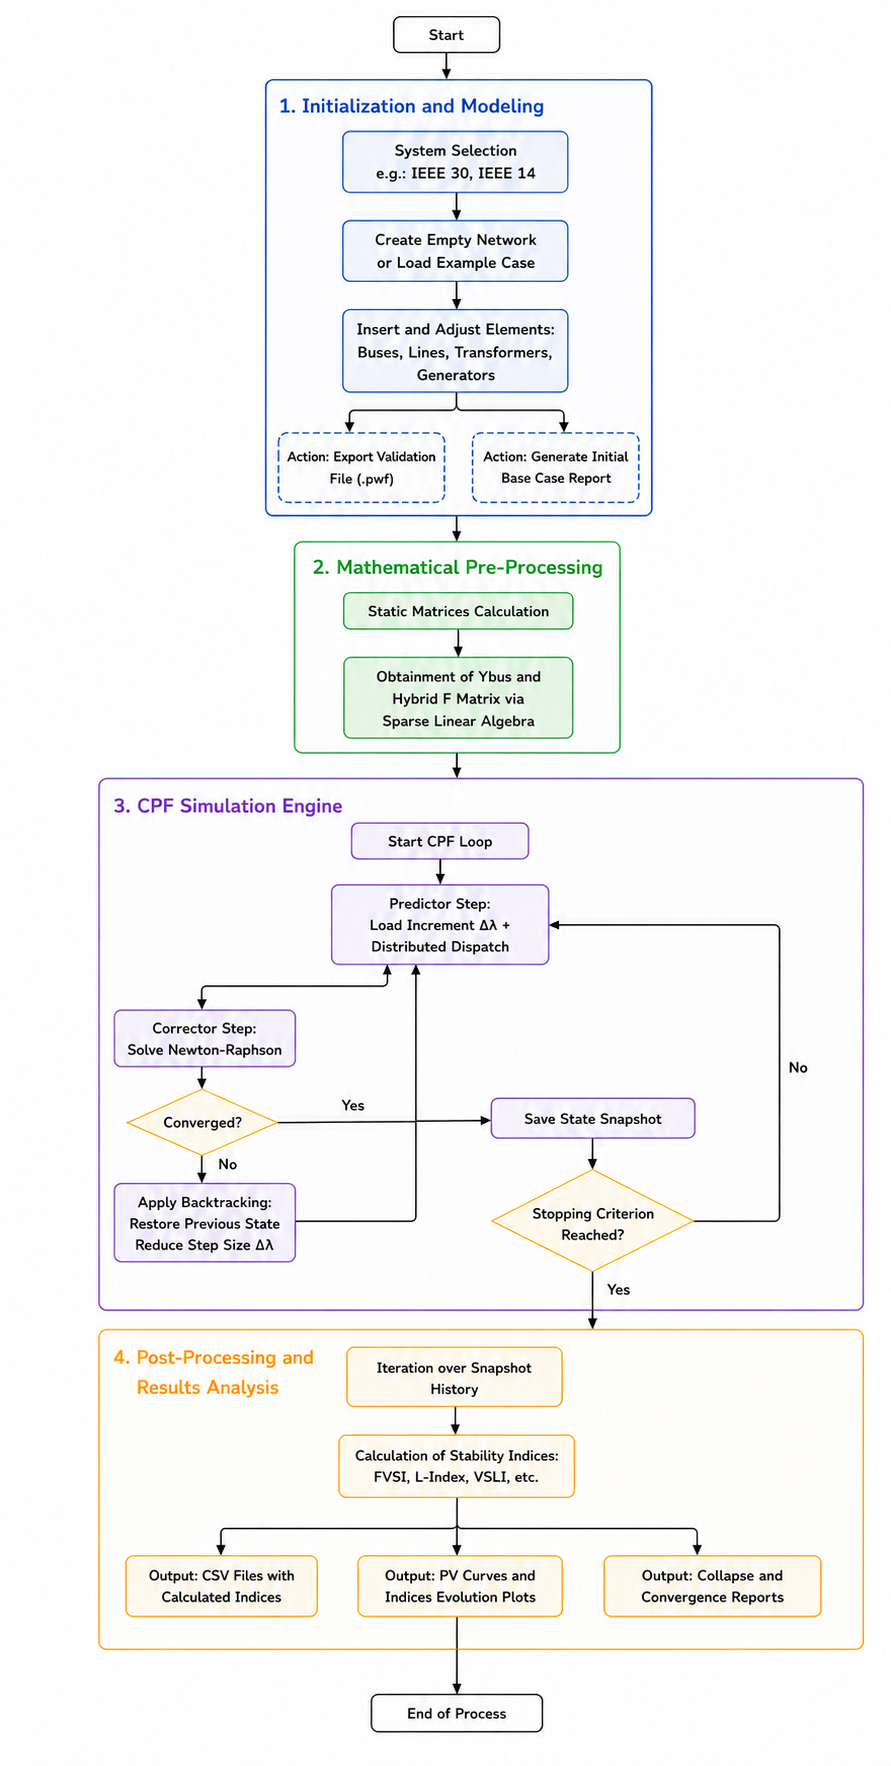
\includegraphics[width=\linewidth]{figures/fluxograma.png}
    \caption{Flowchart detailing the computational architecture and execution steps of the Continuation Power Flow algorithm, from system initialization to post-processing reports.}
    \label{fig:fluxograma}
\end{figure}

\subsection{Optimized Calculation of Indices}
To optimize computational performance, especially for the calculation of indices that depend on matrix inversion (such as the L-Index), sparse linear algebra (\textit{scipy.sparse}) was utilized. The admittance matrices ($Y_{bus}$) and the hybrid matrix $F$ are pre-calculated only once based on the network topology and reused at each step of the simulation. This allows the efficient processing of thousands of loading scenarios in a few seconds, enabling near real-time analysis.

\subsection{System Modeling}

The analysis was primarily carried out on the IEEE 30-bus ANAREDE Equivalent system, ensuring parity with the reference \cite{madureira2023avaliacao}. The adopted premises were:
\begin{itemize}
    \item \textbf{Distributed Dispatch:} The active load increment is distributed proportionally among active generators (G1=86.7\%, G2=13.3\%), according to the DGER configuration of ANAREDE.
    \item \textbf{Reactive Limits:} Reactive generation limits were relaxed ($Q_{lim}$ inactive) to determine the maximum theoretical transmission margin.
    \item \textbf{Load:} Simultaneous increment of P and Q (constant power factor).
\end{itemize}

\autoref{fig:ieee30} shows the diagram of the IEEE 30-bus system used in this work. 

\begin{figure}[htbp]
    \centering
    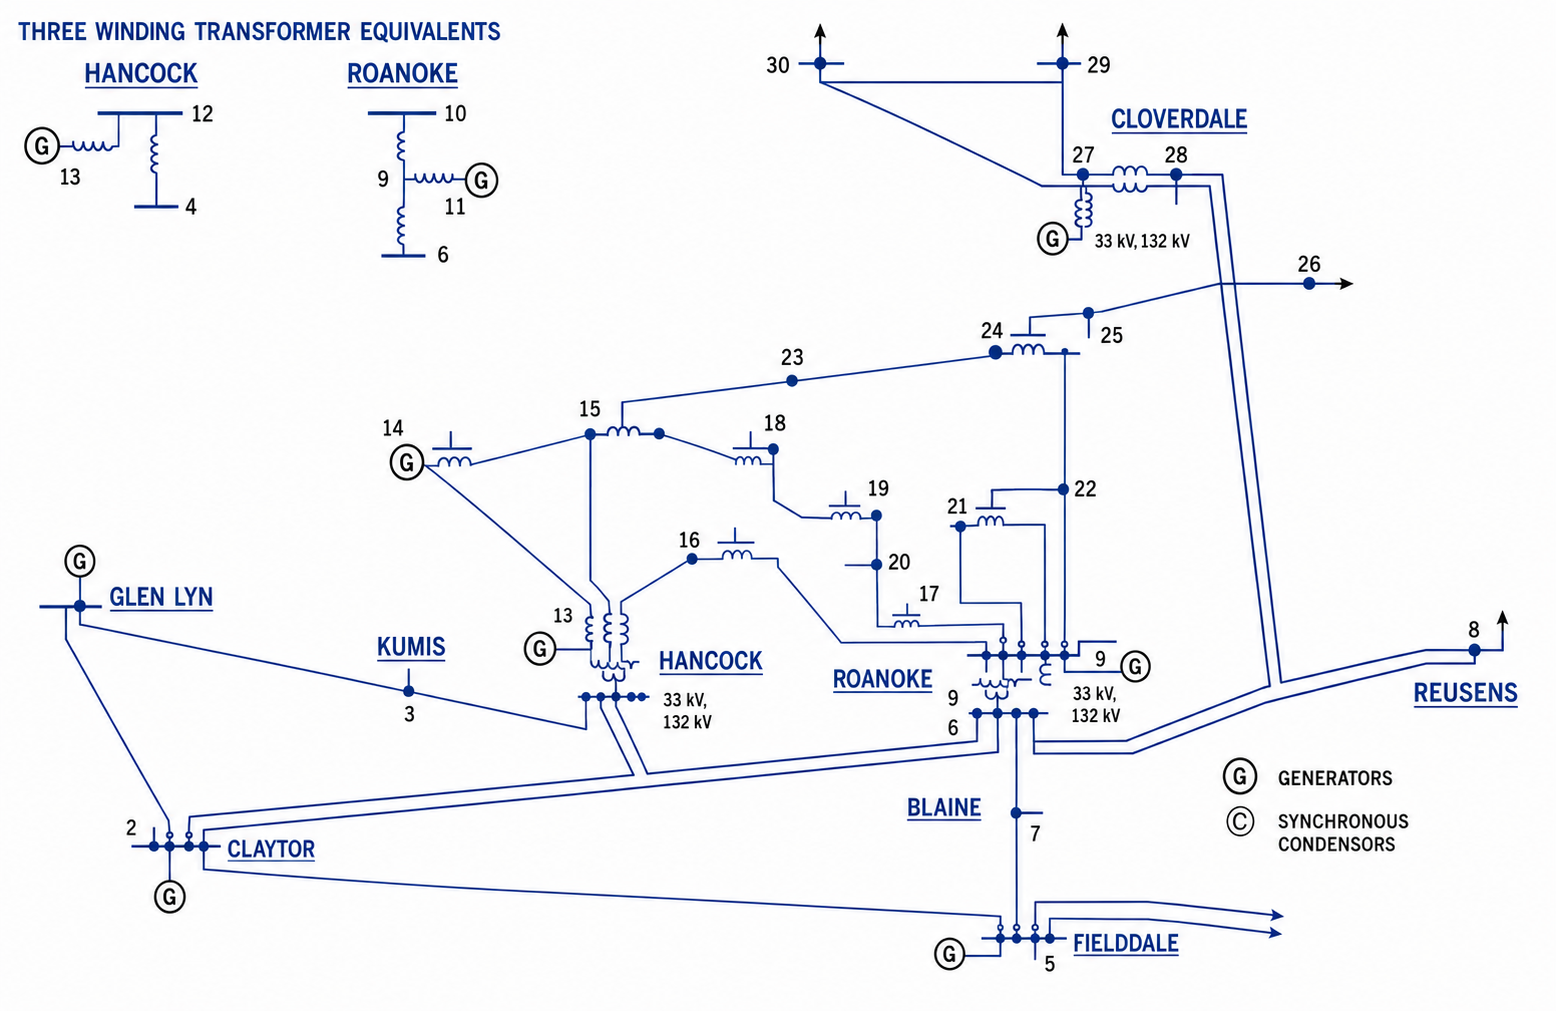
\includegraphics[width=\linewidth]{figures/ieee30bus.png}
    \caption{Single-line diagram of the standard IEEE 30-bus test system utilized for validation against ANAREDE \cite{totonchi}.}
    \label{fig:ieee30}
\end{figure}

To broaden the scope of the study and verify the algorithm's capability across different grid structures, the IEEE 39-bus New England system was also incorporated as a secondary test case. The IEEE 39-bus network is widely known for its heavily meshed structure and robust generation distribution.

\begin{figure}[htbp]
    \centering
    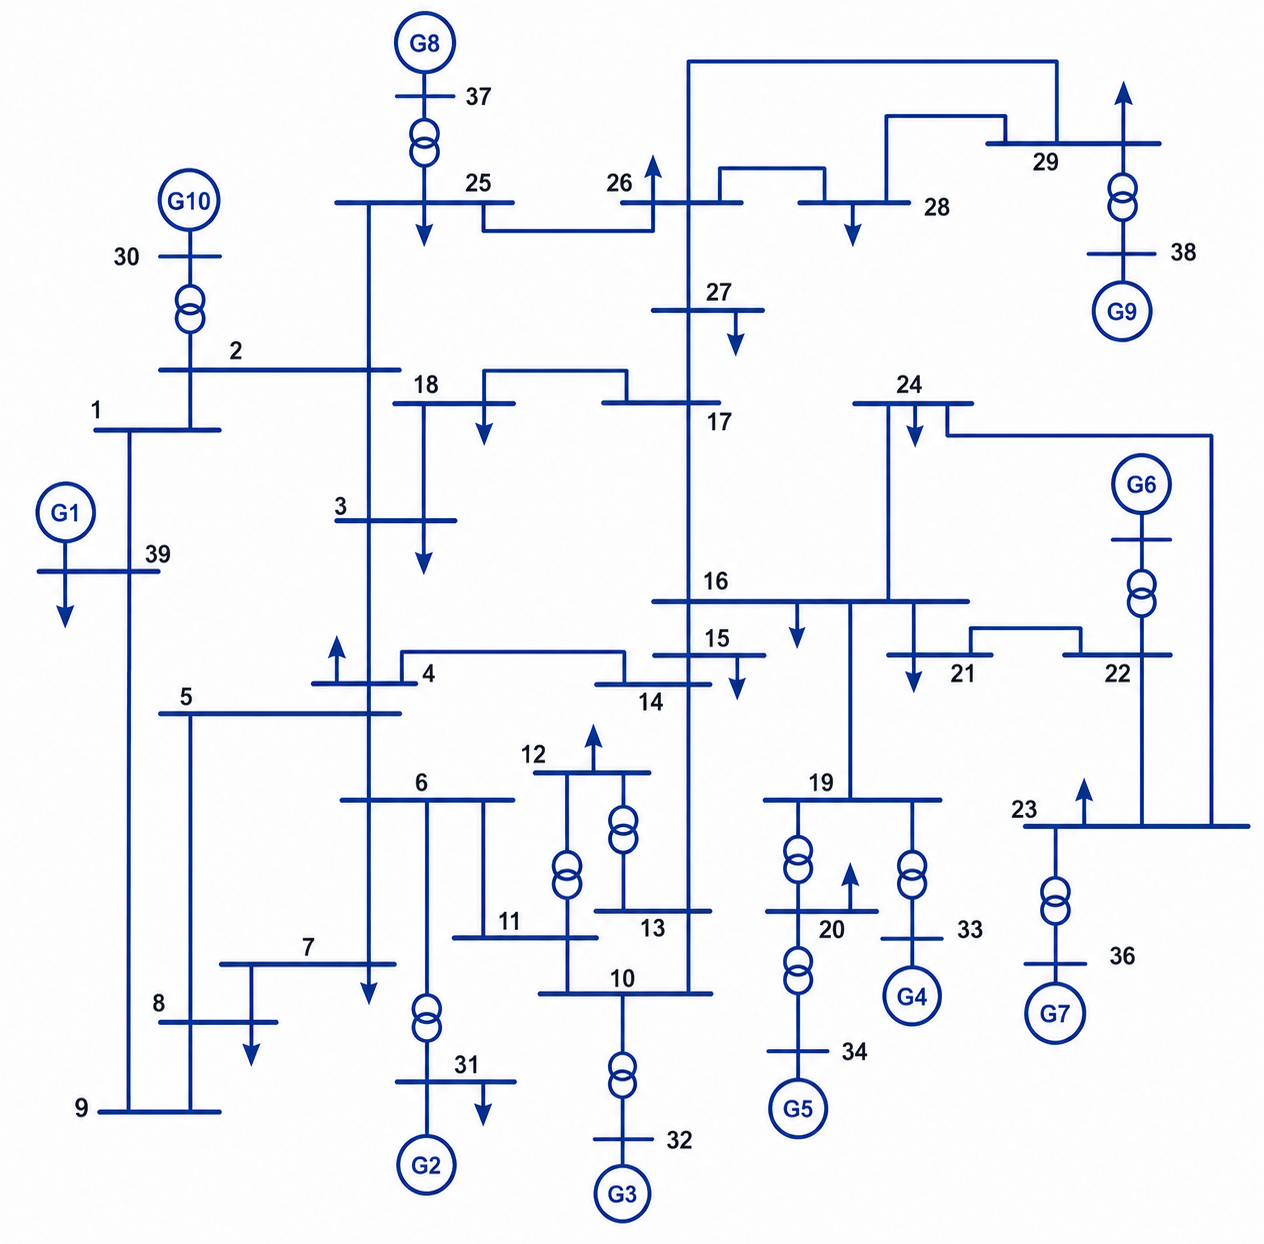
\includegraphics[width=\linewidth]{figures/ieee39bus.png}
    \caption{Single-line diagram of the highly meshed IEEE 39-bus New England test system, used to evaluate index behavior in robust grid topologies.}
    \label{fig:ieee39}
\end{figure}

\section{Results and Discussion}
\label{sec:results}

\subsection{Stability Margin (IEEE 30-Bus)}
The simulation reached the point of collapse with a total loading of 838.50 MW ($\bm{\lambda} \approx 2.95$). This value is extremely close to the 836 MW reported in the reference study \cite{madureira2023avaliacao}, representing a marginal difference of approximately 0.3\%. Thus, the proposed algorithm was able to identify a higher maximum power transfer than the ANAREDE software in the same system. This is important because operation centers need reliable information on the safety and stability limits of the system.

This small discrepancy is attributed to intrinsic differences between the numerical methods of the solvers (Newton-Raphson implementation in Pandapower vs. ANAREDE) and convergence tolerances, rather than modeling errors, given that the base case was accurately validated.

The full trajectory of voltages up to the collapse can be visualized in \autoref{fig:curvapv}. The adaptive step size algorithm allowed for a smooth tracking of the curve, reducing the step automatically as it approached the singularity.

\begin{figure}[htbp]
    \centering
    \includesvg[width=\linewidth]{outputs/ieee_30_anarede_pwf_tcc/pv_figures/curva_pv_sistema_30}
    \caption{PV curves of the IEEE 30-bus system simulated via the developed Python tool, highlighting the critical collapse threshold at 838.5 MW.}
    \label{fig:curvapv}
\end{figure}

For visual comparison purposes, \autoref{fig:curvapv_ref} displays the original curve obtained via ANAREDE in the reference study. A high similarity in the voltage degradation profile is observed, confirming that Bus 30 is the most critical point in the system for both software applications.

\begin{figure}[htbp]
    \centering
    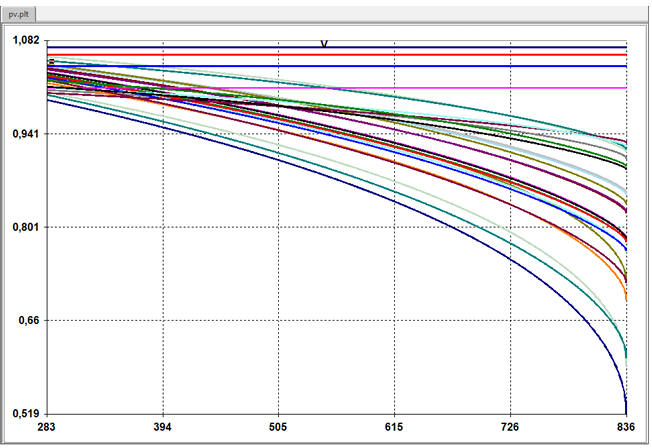
\includegraphics[width=\linewidth]{figures/curva_pv_madureira_ref.png} 
    \caption{Reference PV curve trajectory generated by the ANAREDE software, validating the collapse point observed in the Python simulation \cite{madureira2023avaliacao}.}
    \label{fig:curvapv_ref}
\end{figure}

\subsection{Convergence Analysis and Final State (IEEE 30-Bus)}
The robustness of the implemented algorithm can be observed through the Convergence Report automatically generated by the tool. \autoref{tab:convergencia} presents the final iterations of the process, demonstrating the operation of the step refinement mechanism (\textit{backtracking}).

\begin{table}[htbp]
\centering
\caption{Summary of the Final Iterations from the Convergence Report}
\label{tab:convergencia}
\begin{tabular}{llccr}
\toprule
\textbf{Iter} & \textbf{Status} & \textbf{Step} & $\bm{\lambda}$ \textbf{(Total)} & \textbf{Load (MW)} \\ \midrule
... & ... & ... & ... & ... \\
985 & Converged & 0.0125 & 2.9586 & 838.47 \\
986 & \textbf{Divergent} & 0.0125 & 2.9711 & --- \\
987 & Converged & 0.0063 & 2.9649 & 838.49 \\
989 & Converged & 0.0031 & 2.9617 & 838.50 \\
990 & \textbf{Divergent} & 0.0031 & 2.9649 & --- \\ \bottomrule
\end{tabular}
\end{table}

It can be observed that upon reaching the load of 838.47 MW (Iteration 985), the step of 0.0125 p.u. leads to divergence (Iteration 986). The algorithm then backtracks and attempts a smaller step size (0.0063), managing to converge slightly further (838.49 MW), until reaching the precision limit.

The Collapse Report revealed that, at the final instant of the simulation, the voltage at Bus 30 reached the critical value of 0.5210 pu, with an extremely wide phase angle of -81.64 degrees. Bus 29, which is electrically close, stood at 0.5946 pu. This voltage profile confirms that the collapse occurred due to the exhaustion of reactive power transmission capacity to that region of the network, characterizing a local stability problem that evolved into a system collapse.

\subsection{Comparative Analysis of Indices (IEEE 30-Bus)}

The indices were calculated for the entire trajectory. \autoref{fig:indices_fvsi} presents the FVSI index. It is noted that it saturates quickly in lines near generation units (Lines 1, 2, and 4), indicating high stress in reactive power transport.

\begin{figure}[htbp]
    \centering
    \includesvg[width=\linewidth]{outputs/ieee_30_anarede_pwf_tcc/index_figures/analise_fvsi_30}
    \caption{Evolution of the FVSI line index in the IEEE 30-bus system, capturing the rapid saturation and severe reactive stress on generation outlet lines.}
    \label{fig:indices_fvsi}
\end{figure}

The $L_{mn}$ index (\autoref{fig:indices_lmn}) confirms this diagnosis, presenting critical values ($>0.8$) for the same lines in the 95\% loading scenario.

\begin{figure}[htbp]
    \centering
    \includesvg[width=\linewidth]{outputs/ieee_30_anarede_pwf_tcc/index_figures/analise_lmn_30}
    \caption{Progression of the $L_{mn}$ line index across loading scenarios in the IEEE 30-bus system, corroborating the critical lines identified by the FVSI.}
    \label{fig:indices_lmn}
\end{figure}

The NLSI (\autoref{fig:indices_nlsi}) and NVSI (\autoref{fig:indices_nvsi}) indices proved to be more sensitive, with several elements exceeding the 1.0 limit in the critical scenario, suggesting a more conservative assessment of stability.

\begin{figure}[htbp]
    \centering
    \includesvg[width=\linewidth]{outputs/ieee_30_anarede_pwf_tcc/index_figures/analise_nlsi_30}
    \caption{Behavior of the NLSI line index, highlighting multiple components reaching critical thresholds in the 95\% loading scenario.}
    \label{fig:indices_nlsi}
\end{figure}

\begin{figure}[htbp]
    \centering
    \includesvg[width=\linewidth]{outputs/ieee_30_anarede_pwf_tcc/index_figures/analise_nvsi_30}
    \caption{Sensitivity and profile of the NVSI line index relative to apparent power variations in the IEEE 30-bus system.}
    \label{fig:indices_nvsi}
\end{figure}

Finally, the L-Index (\autoref{fig:indices_lindex}) correctly identified distant load buses (such as Bus 30) as the weakest points in the network (values close to 1), complementing the insights gained from the line indices.

\begin{figure}[htbp]
    \centering
    \includesvg[width=\linewidth]{outputs/ieee_30_anarede_pwf_tcc/index_figures/analise_l_index_30}
    \caption{Evaluation of the nodal L-Index in the IEEE 30-bus system, accurately pinpointing the structural vulnerability of critical load buses (e.g., Bus 30).}
    \label{fig:indices_lindex}
\end{figure}

Furthermore, there is an interesting point regarding this index. It was observed that at the most critical bus found, the index value decreased as the loading increased. This differs from the behavior of all other buses. Since this specific index was not mentioned in \cite{madureira2023avaliacao}, it is not entirely clear whether this result accurately reflects the system's reality, but it remains a curious finding to observe.

\subsection{Application and Comparison: IEEE 39-Bus System}
To evaluate how network topology impacts the predictive capacity of stability indices, the same CPF algorithm was applied to the IEEE 39-bus New England system. Unlike the 30-bus network, which presents radial-like weak corridors, the 39-bus system is heavily meshed and supported by a larger number of generation units. This evaluation serves to test the algorithm's standalone robustness without directly comparing it to ANAREDE.

\textbf{1. PV Curve Behavior and Stability Margin:}
While the IEEE 30-bus system showed a steep, distinct ``nose'' curve for its weakest bus (\autoref{fig:curvapv}), the PV curves generated for the IEEE 39-bus system exhibited a more uniform and gradual voltage degradation across multiple load buses prior to collapse. The strong meshing allowed active power to be rerouted efficiently, pushing the Maximum Loading Point (MLP) to a significantly higher load margin. Specifically, the system safely evolved from a base load of 6,254.23 MW to an impressive collapse threshold of 13,357.13 MW ($\bm{\lambda} = 2.1357$), representing a load increase capability of over 113.5\%. At the bifurcation point, Bus 6 was identified as the critical node, reaching a minimum voltage of 0.6629 pu.

\begin{figure}[htbp]
    \centering
    \includesvg[width=\linewidth]{outputs/ieee_39_barras_new_england/pv_figures/curva_pv_sistema_39}
    \caption{PV curves of the IEEE 39-bus New England system, demonstrating a more uniform and resilient voltage degradation profile due to its highly meshed topology.}
    \label{fig:curvapv_39}
\end{figure}

The robustness of the developed backtracking algorithm was heavily tested in this meshed topology. The convergence report indicates that the simulation required 581 iterations to reach the singularity, dynamically reducing the increment step size from an initial $0.2000$ pu down to a highly precise $0.0008$ pu in the final divergent iterations. This ensures the MLP was pinpointed with exact precision rather than a premature numerical divergence.

\textbf{2. Response of Line Indices (FVSI, $L_{mn}$, NLSI, NVSI):}
As previously shown, in the IEEE 30-bus system, line indices saturated quickly and presented sharp spikes near generation outlet lines. Conversely, when calculated for the IEEE 39-bus system (\autoref{fig:indices_fvsi_39}, \autoref{fig:indices_lmn_39}, \autoref{fig:indices_nlsi_39}, \autoref{fig:indices_nvsi_39}), the exact same indices displayed a much broader distribution of stress. 

\begin{figure}[htbp]
    \centering
    \includesvg[width=\linewidth]{outputs/ieee_39_barras_new_england/index_figures/analise_fvsi_39}
    \caption{Evolution of the FVSI line index in the IEEE 39-bus system, showcasing how meshed topologies distribute reactive stress across multiple transmission corridors.}
    \label{fig:indices_fvsi_39}
\end{figure}

\begin{figure}[htbp]
    \centering
    \includesvg[width=\linewidth]{outputs/ieee_39_barras_new_england/index_figures/analise_lmn_39}
    \caption{Progression of the $L_{mn}$ line index in the IEEE 39-bus system, reflecting a distributed burden rather than localized bottlenecks.}
    \label{fig:indices_lmn_39}
\end{figure}

\begin{figure}[htbp]
    \centering
    \includesvg[width=\linewidth]{outputs/ieee_39_barras_new_england/index_figures/analise_nlsi_39}
    \caption{Response of the NLSI line index to loading increments, highlighting shared transmission burdens across the IEEE 39-bus grid.}
    \label{fig:indices_nlsi_39}
\end{figure}

\begin{figure}[htbp]
    \centering
    \includesvg[width=\linewidth]{outputs/ieee_39_barras_new_england/index_figures/analise_nvsi_39}
    \caption{Evolution of the NVSI index in the IEEE 39-bus system, illustrating the distributed impact of apparent power variations.}
    \label{fig:indices_nvsi_39}
\end{figure}

Rather than a few lines peaking abruptly, multiple interconnected components experienced a simultaneous, gradual rise in their index values. The power flow report near the collapse point corroborates this, revealing severe and distributed loading across critical corridors, such as Transformer 2-9 (242.8\% loaded) and Line 21-15 (201.6\% loaded). This demonstrates that in highly meshed networks, line indices may be less effective at pinpointing a single point of failure, as the network tends to distribute the burden and collapse holistically rather than locally.

\textbf{3. Response of Nodal Indices (L-Index):}
In contrast to the line indices, the L-Index proved to be consistently reliable across both topologies. Just as it correctly identified the weakest node in the 30-bus network, the L-Index successfully highlighted the most vulnerable load buses in the 39-bus system (\autoref{fig:indices_lindex_39}) as it approached the MLP, demonstrating its analytical robustness regardless of grid meshing. It is important to note that buses connected to generators were not considered in this index.

\begin{figure}[htbp]
    \centering
    \includesvg[width=\linewidth]{outputs/ieee_39_barras_new_england/index_figures/analise_l_index_39}
    \caption{Nodal vulnerability mapping using the L-Index in the complex IEEE 39-bus topology, maintaining predictive accuracy regardless of grid meshing.}
    \label{fig:indices_lindex_39}
\end{figure}

\section{Conclusions}
\label{sec:conclusions}

This work presented the development of a Python-based computational tool for voltage stability assessment, incorporating a Continuation Power Flow algorithm with adaptive step refinement and distributed dispatch, in order to faithfully reproduce the methodology utilized by the ANAREDE software. The validation performed on the IEEE 30-bus system demonstrated excellent agreement between the solutions, with the maximum loading margin (836 MW in \cite{madureira2023avaliacao} and 838.50 MW) being obtained almost precisely, confirming the consistency of the proposed modeling and implementation.

The comparative analysis of stability indices revealed that each metric responds to distinct mechanisms associated with voltage collapse. The line indices (FVSI, $L_{mn}$, NLSI, NVSI) proved effective in identifying local overloads and transmission bottlenecks, highlighting elements that limit reactive power transfer along the CPF trajectory. On the other hand, the nodal L-Index exhibited a strong correlation with the system's critical point, clearly capturing the structural weakness of load buses. 

Furthermore, the expansion of the study to the highly meshed IEEE 39-bus New England system emphasized the impact of grid topology on these indices. While line indices offer sharp predictions in weaker, radial-leaning networks, they tend to display distributed stress in heavily meshed grids. 

The results demonstrate that no single index is capable of fully characterizing the phenomenon; however, the combined use of line and bus metrics provides a complementary and comprehensive view of the network's behavior. The developed tool integrates these indicators consistently, establishing itself as a robust platform for stability studies, planning, and the development of control strategies.

\section{Future Work}
\label{sec:future}

As perspectives for the continuity of this work, several extensions can be explored to expand the applicability of the developed tool. A primary development involves the incorporation of new voltage stability indices, especially those focused on nodal evaluation, such as VCPI$_{bus}$, SDC, SVSI, among others \cite{modarresi2016comprehensive}. The inclusion of these metrics will allow for a more comprehensive comparison of the performance of different indicators, evaluating their sensitivity, robustness, and ability to anticipate the maximum loading point under varying operational conditions.

Another important evolutionary path is the application of the methodology in contingency scenarios, particularly in N-1 analyses or even multiple contingencies, which could evolve into Power System Reliability studies. Replicating the continuation power flow under these conditions will allow for investigating how the loss of lines, transformers, or generating units affects the voltage stability margin, providing a more realistic view of the system's vulnerabilities. This type of study is fundamental for operational security assessments and planning, especially in systems with radial topologies or regions highly dependent on transmission.

Finally, a promising directive involves the implementation and analysis of mechanisms aimed at increasing the Voltage Stability Margin. Among these, reactive reinforcements can be considered, such as capacitor banks and shunt compensators, transformers with adjustable TAP, FACTS devices (like SVCs and STATCOMs), alongside optimized generation redispatch strategies. Re-executing the CPF following the introduction of these resources will allow for quantifying the effective margin gain and determining which interventions present the best ratio between efficacy and control effort.

These investigative lines not only expand the tool's capacity but also align the study more closely with real-world operational and planning demands, particularly in modern systems increasingly subjected to narrow stability limits and elevated power flows.

\bibliographystyle{IEEEtran}
\bibliography{biblio}

\begin{IEEEbiography}[{
\includegraphics[width=1in,height=1.25in,clip,keepaspectratio]{figures/photoGoncalo.png}}]{Gonçalo Fontenele} (ORCID: 0009-0008-1378-1420) earned, from the Universidade Federal do Rio de Janeiro (UFRJ), a BSc in Electrical Engineering and is currently pursuing his MSc in Electrical Engineering at COPPE/UFRJ. He serves as an Industrial Data Analyst, working with energy generation and transmission companies to increase the reliability and performance of assets through real-time data analysis. His work in Power System Reliability has resulted in peer-reviewed conference publications, software development, and technical projects. His research interests include Renewable Energy, Photovoltaic Systems, Power System Reliability, and Climate Resilience.
\end{IEEEbiography}

\begin{IEEEbiography}[{
\includegraphics[width=1in,height=1.25in,clip]{figures/photoLeonardo.jpg}}]{Leonardo R. B. Campos} received the B.Sc. degree in electrical engineering from the Federal University of Rio de Janeiro (UFRJ), Rio de Janeiro, Brazil.

He is currently pursuing the M.Sc. degree at COPPE/UFRJ, Rio de Janeiro, Brazil, as a researcher with the Laboratory of Alternative Energy Sources (LAFAE). His primary research focus is on power system stability, control, and computational optimization.
\end{IEEEbiography}

\begin{IEEEbiography}[{
\includegraphics[width=1in,height=1.25in,clip,keepaspectratio]{figures/photoMurilo.jpg}}]{Murilo E. C. Bento}(Member, IEEE) received the B.Sc., M.Sc., and Ph.D degrees in electrical engineering from the University of São Paulo (USP), São Carlos, Brazil, in 2013, 2016, and 2020, respectively. 
	
	He is currently an Adjunct Professor with the Federal University of Rio de Janeiro (UFRJ), Rio de Janeiro, Brazil. His research focuses on power system stability analysis and control, with emphasis on small-signal and voltage stability problems. He is an Associate Editor of the journal \emph{Electricity} (MDPI) and the journal \emph{Electrical Engineering} (Springer).
\end{IEEEbiography}

\EOD

\end{document}